\documentclass[border=2pt]{standalone}
\usepackage[dvipsnames,svgnames,x11names]{xcolor}
\usepackage{tikz}
\usetikzlibrary{arrows.meta,positioning,shapes.geometric}
\begin{document}
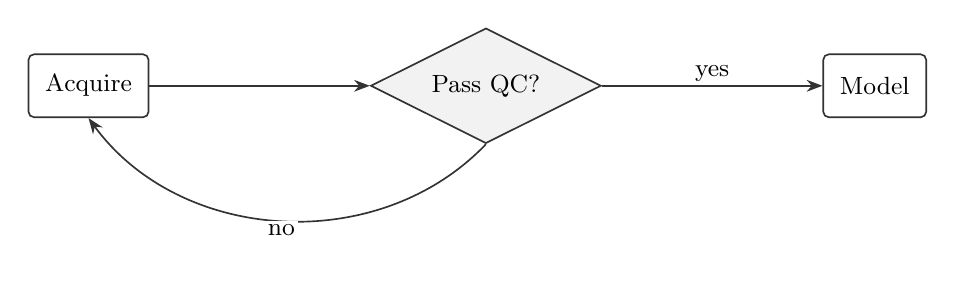
\begin{tikzpicture}[font=\small,>=Stealth]
\node[rectangle,rounded corners=2pt,fill=white,draw=black!80,text=black,line width=0.6pt,minimum height=8mm,inner xsep=6pt,inner ysep=4pt,align=center] (collect) at (0,0) {Acquire};
\node[diamond,aspect=2,fill=black!5,draw=black!80,text=black,line width=0.6pt,minimum height=8mm,inner xsep=6pt,inner ysep=4pt,align=center,right=28mm of collect] (check) {Pass QC?};
\node[rectangle,rounded corners=2pt,fill=white,draw=black!80,text=black,line width=0.6pt,minimum height=8mm,inner xsep=6pt,inner ysep=4pt,align=center,right=28mm of check] (model) {Model};
\draw[->,draw=black!80,line width=0.6pt] (collect) -- (check);
\draw[->,draw=black!80,line width=0.6pt] (check) -- node[pos=0.5,above,fill=white,inner sep=1.2pt] {yes} (model);
\draw[->,draw=black!80,line width=0.6pt] (check.south) to[bend left=50] node[pos=0.5,below,fill=white,inner sep=1.2pt] {no} (collect.south);
\end{tikzpicture}
\end{document}
